\begin{chapter}{Testes e Resultados}
O perfil dos participantes que aceitaram realizar testes com o protótipo
desenvolvido neste trabalho, bem como o ambiente onde os testes ocorreram, serão
apresentados neste capítulo. Os objetivos das tarefas elaboradas para ser
realizado pelos participantes assim como o \textit{software} utilizado  para
controlar o cursor do mouse também serão mostrados. Por último será apresentado
os resultados quantitativo e qualitativo do teste.  

\begin{section}{Perfil dos Voluntários}
O estudo foi realizado com 7 pessoas do sexo masculino e 3 pessoas do sexo
feminino, totalizando 10 participantes, com idades que variaram de 21 a 28 anos.
Todos eles são estudantes de graduação ou pós-graduação da Universidade Federal
do pará (UFPA). O único critério exigido para participar dos testes era que o
participante deviria ter familiaridade com os \textit{websites} utilizados nas
tarefas do teste.  

A seleção dos voluntários ocorreu através da abordagem ao participante do
experimento convidando-o a realizar o teste aplicado neste trabalho. Após a
aceitação do participante, foi então apresentado o trabalho desenvolvido,
demonstrando a motivação do estudo, todos os objetivos, o tempo médio da duração
do teste e  as etapas de cada tarefa que seria realizada. 

Logo após a apresentação do trabalho o voluntário deveria ler o TCLE (Termo de
Consentimento Livre e Esclarecido), onde foi estabelecido, que ao assinar o
termo, o participante declarava estar ciente de que os dados coletados nos
testes seriam utilizados para fins de pesquisa acadêmica. Este termo deixa
claro o objetivo do trabalho, informando alguns pontos sobre a restrição dos
dados do participante e declarando por fim que o participante aceitaria os
termos. O termo apresentado para assinatura do participante é demonstrado no
Apêndice A – Termo de consentimento de livre e esclarecido. Ao assinar o TCLE o
voluntário estava habilitado a realizar as tarefas elaboradas. 
\end{section}

\begin{section}{Ambientes de Testes e Procedimentos}

O ambiente os testes foram realizados é mostrado na Figura~\ref{fig:ambiente}.
Como pode ser visto, uma \textit{webcam} foi posicionada em frente do usuário. O
dispositivo de sopro desenvolvido foi fixado próximo a boca do usuário graças a
ajuda de um fone de ouvido modificado que serviu de suporte que, independente da
posição da cabeça do usuário, o suporte sempre mantinha o dispositivo de sopro
em frente a boca do participante.

\begin{figure}[!h]
	\centering
	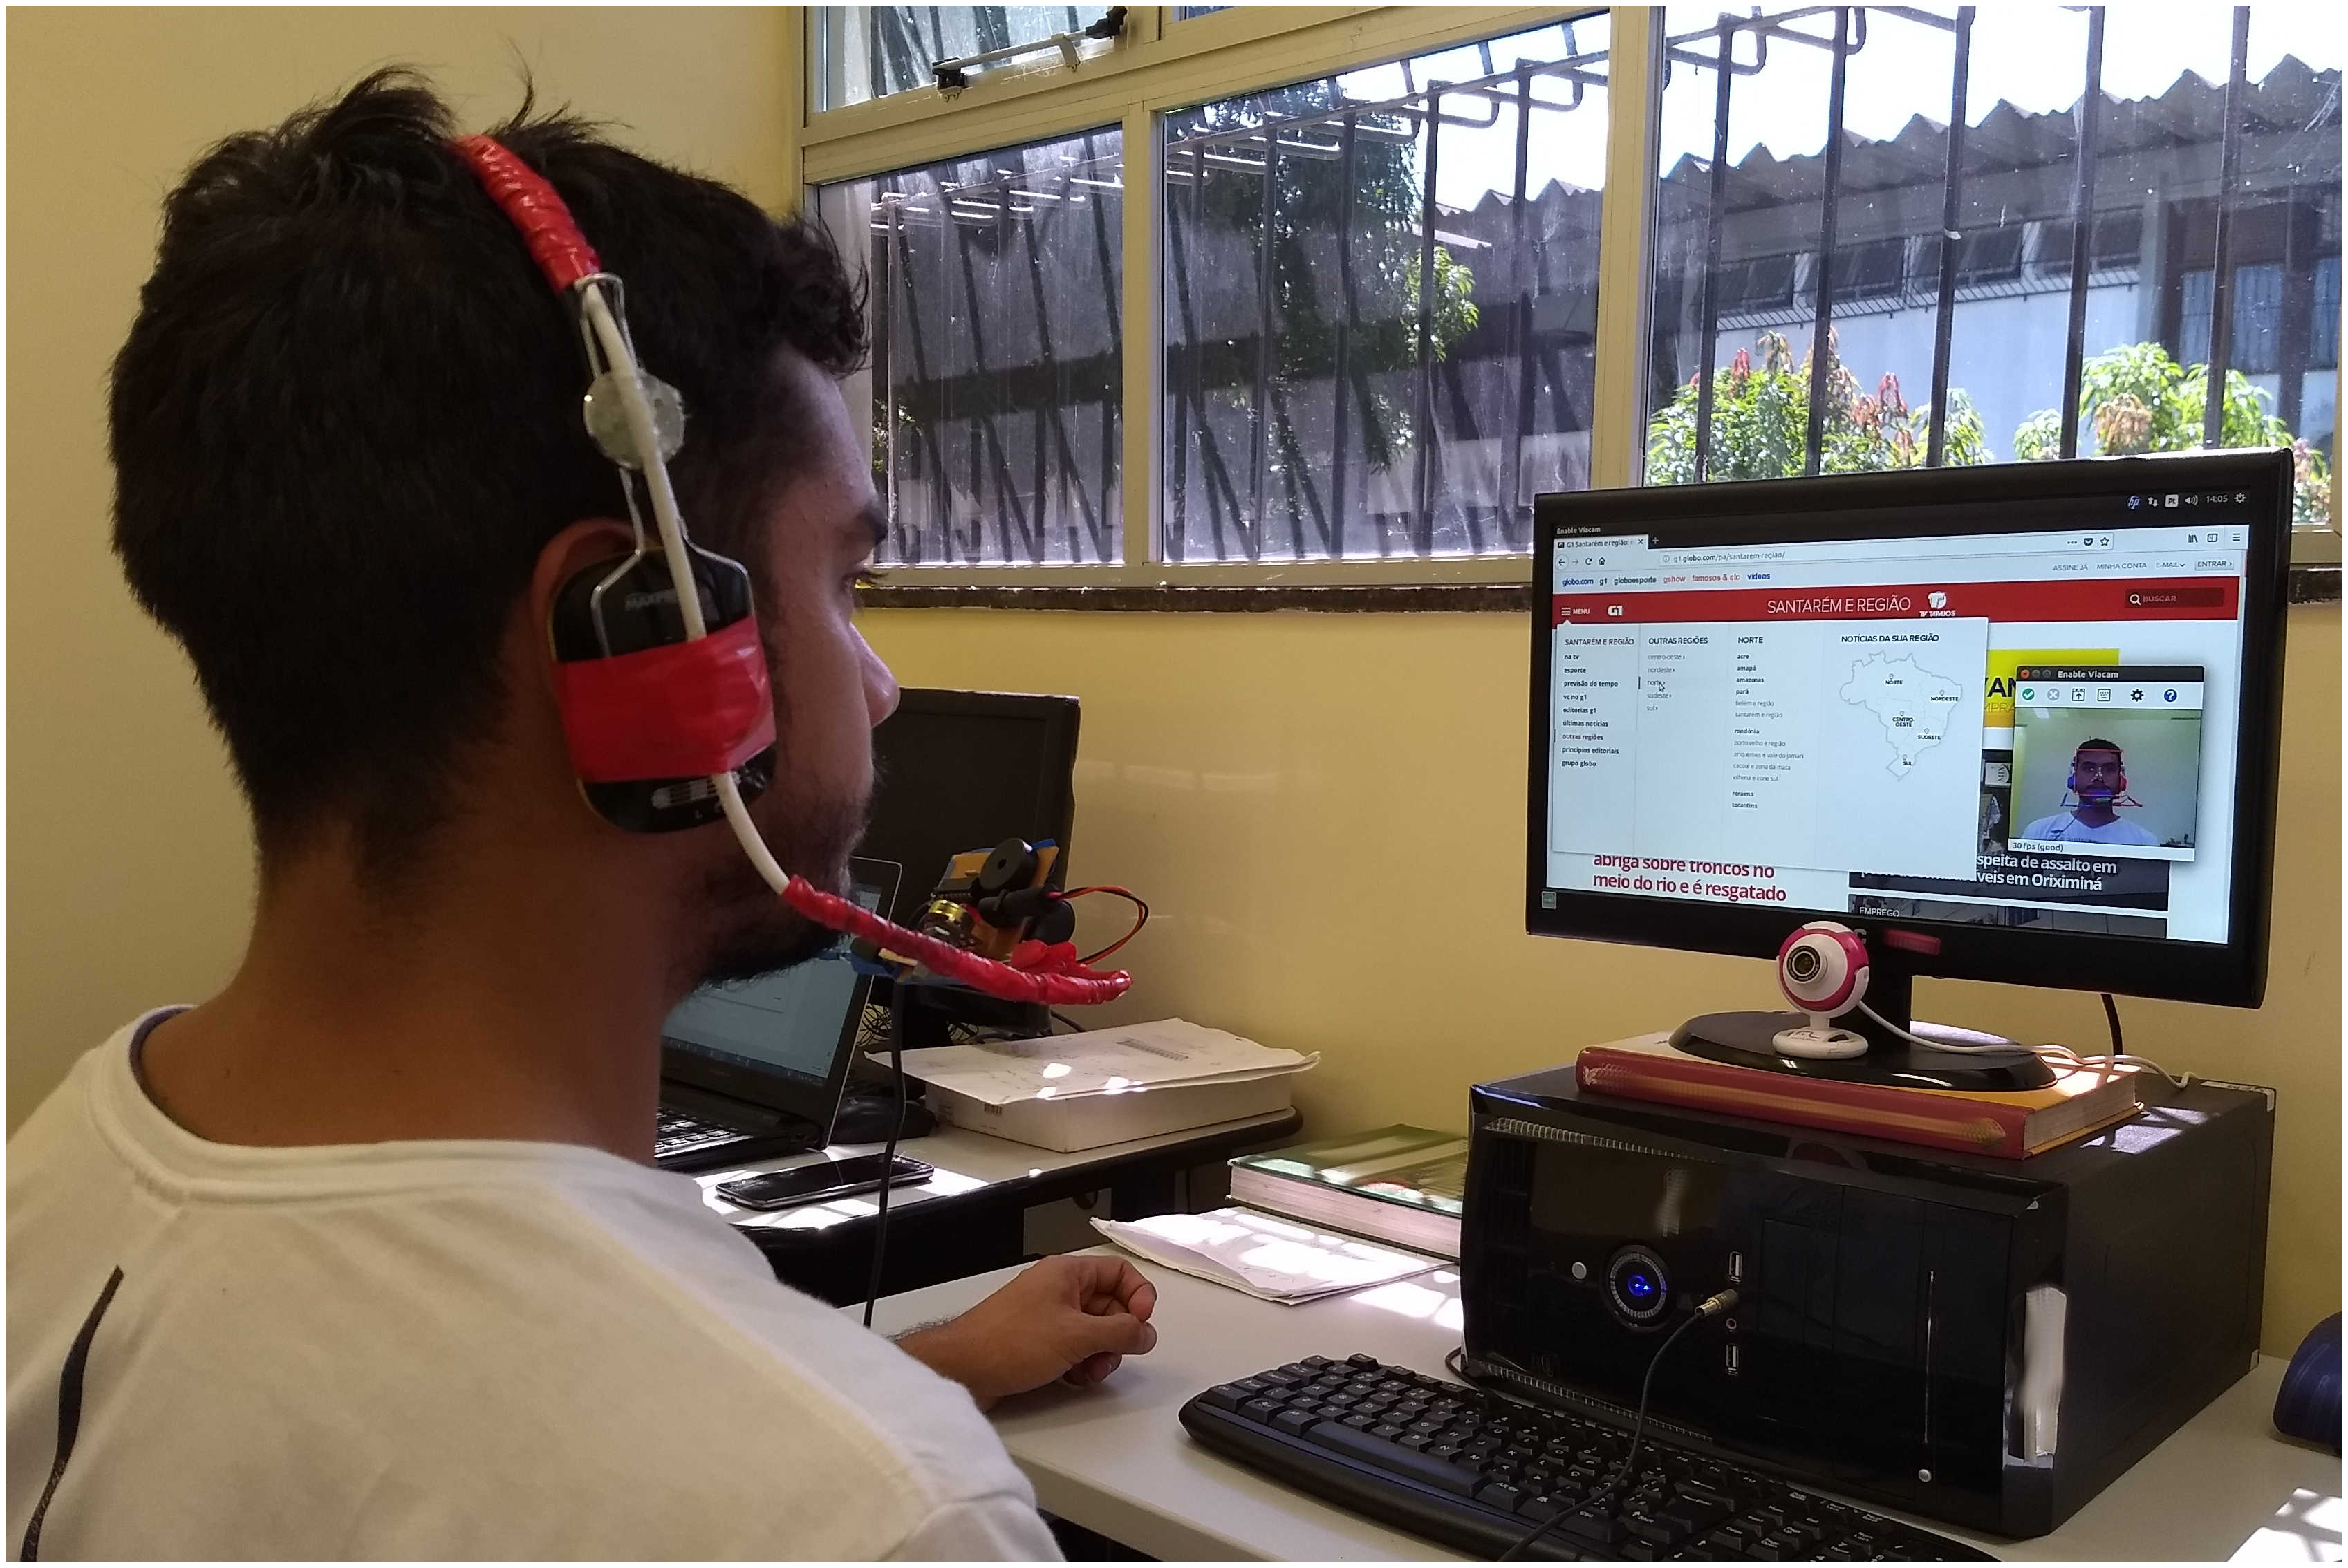
\includegraphics[width=1.00\linewidth]{fig/denes}
	\caption{Um usuário realizando as tarefas no ambiente de teste.}
	\label{fig:ambiente}
\end{figure}

Os testes foram realizados individualmente com todos os participante durante a
luz do dia. Todos estavam devidamente acomodados em uma cadeira com apoio para
as mãos e costas. A iluminação do ambiente foi totalmente controlada com a ajuda
de lâmpadas fluorescentes da sala onde foi realizadas os testes e das janelas
translúcidas logo atrás do monitor. 

A computador utilizado possuia um processador Intel Core i5 da 4ª geração e
3.20~GHz, memória RAM de 4~GB e 1~TB de espaço de armazenamento com o sistema
operacional Ubuntu 16.04 Xenial Xerus x64. O monitor era um AOC E1670SWU de LED
com 15.6 polegadas e com resolução de 1366 $\times$ 768.

\begin{figure}[!h]
	\centering
	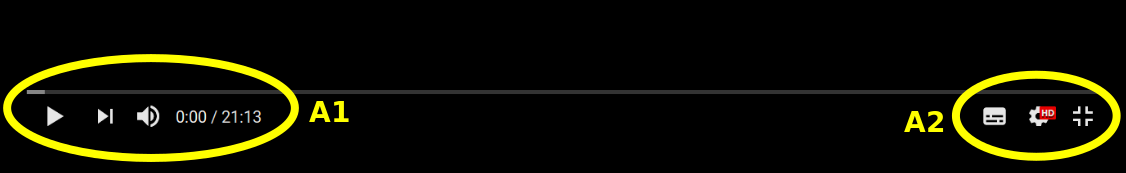
\includegraphics[width=1.00\linewidth]{fig/YT}
	\caption{Regiões de interesse do \textit{website} YouTube.}
	\label{fig:youtube}
\end{figure}

\begin{figure}[!h]
	\centering
	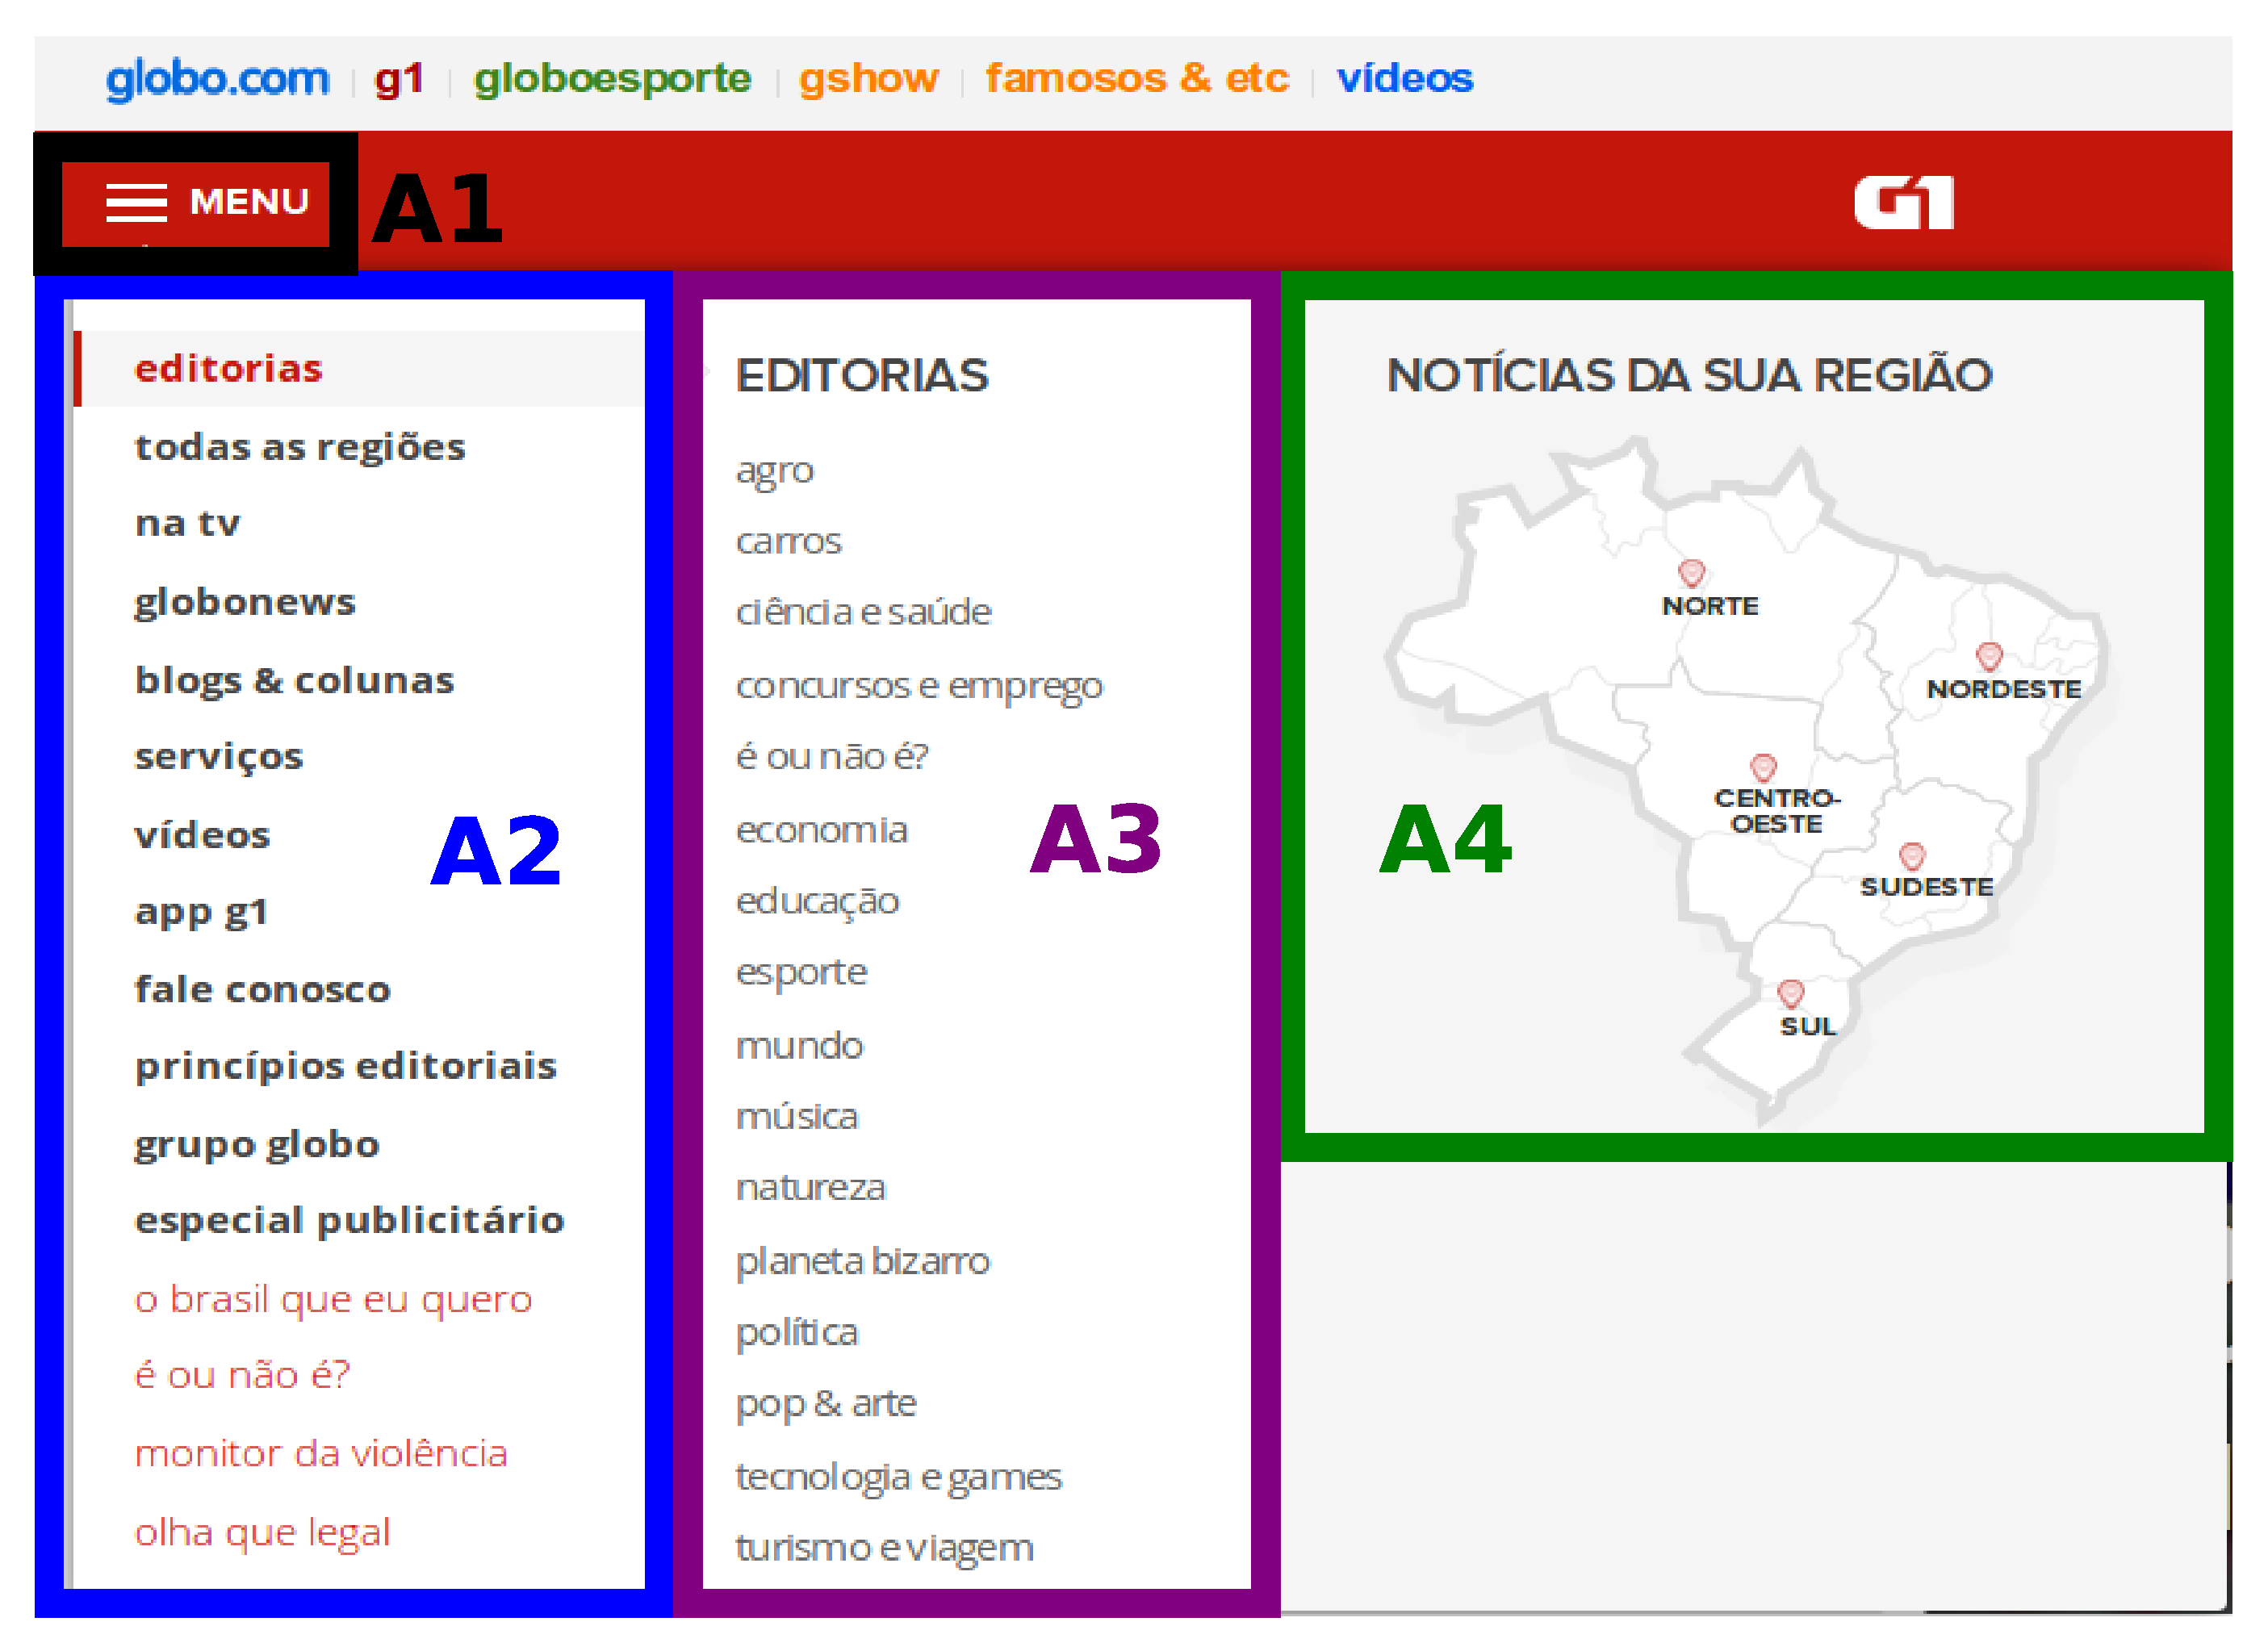
\includegraphics[width=1.00\linewidth]{fig/g1}
	\caption{Regiões de interesse do \textit{website} G1.}
	\label{fig:g1}
\end{figure}

As tarefas dos testes foram realizadas nos \textit{websites} YouTube
(\url{https://www.youtube.com/}) e G1(\url{https://g1.globo.com/}), mostrados
nas Figuras~\ref{fig:youtube} e~\ref{fig:g1}, respectivamente, com suas
respectivas regiões de interesse destacados em retângulos coloridos e nomeados
como A1, A2, etc. Esses \textit{websites} foram escolhidos porque eles não são
adaptados para serem utilizadas por tecnologias alternativas. Quado é utilizado
o \textit{dwell time} como método de clique, por exemplo, assistir um vídeo no
modo de tela cheia no YouTube se torna um desafio, visto que o usuário é forçado
a mover o cursor do \textit{mouse} a todo o momento afim de evitar que a cliques
involuntários ocorram. Já para o G1, o menu interativo é um grande problema para
\textit{software} alternativos de controle do cursor do \textit{mouse}, como o
eViacam, visto que os itens na barra de navegação do menu se expandem
e mudam apenas com o simples ato de passar o ponteiro em cima desses itens.

Por meio de testes exaustivos, verificou-se que o valor que oferece maior
conforto aos usuários ao usar o rastreador de cabeça eViacam é 11 nos eixos X e
Y. Além disso, o tempo de 15 décimos de segundo (ou seja, 1,5 segundo) para o
clique com o \textit{dwell time} foi estabelecido. O valor padrão no eViacam é
de 10 décimos de segundo, porém esse tempo estava demasiadamente rápido, e isso
poderia afetar a experiência do usuário.

Os participantes foram instruídos a seguir a mesma rotina de tarefas utilizando
como método de clique o \textit{dwell time} e com o dispositivo baseado em
sopro. As tarefas mostradas abaixo foram apresentadas aos usuários com uma breve
descrição e em ordem de execução. Os usuários foram convidados a concluir as
tarefas primeiro com o protótipo baseado no sopro e em seguida com o
\textit{dwell time}.  Para o G1, a tarefa se iniciou na página
principal do \textit{website} enquanto que para o YouTube, a tarefa se iniciou
em um vídeo em modo de tela cheia.

\begin{itemize}
\item Teste no YouTube (veja a Figura~\ref{fig:youtube}):
	\begin{itemize}
	\renewcommand\labelitemi{--}
	\item Clicar no botão de play do vídeo.                            \hfill (região A1)
	\item Clicar n botão de ativar a legenda do vídeo.                 \hfill (região A2)
	\item Diminuir o volume em cerca de 50\%.                          \hfill (região A1)
	\item Retroceder o video em exebição para os 10 segundos iniciais. \hfill (região A1)
	\item Clicar no botão de avançar vídeo.                            \hfill (região A1)
	\item Clicar no botão de sair do modo de tela cheia.               \hfill (região A2)
	\end{itemize}
\item Test on G1 webpage (veja a Figura~\ref{fig:g1}):
	\begin{itemize}
	\item[$\ast$] Subtarefa 1:
		\begin{itemize}
		\item[--] Mover o cursor para o ícone de menu.                   \hfill (região A1)
		\item[--] Mover para ``editorias''.                              \hfill (região A2)
		\item[--] Clicar em ``economia''.                                \hfill (região A3)
		\end{itemize}
	\item[$\ast$] Subtarefa 2:
		\begin{itemize}
		\item[--] Mover o cursor para o ícone de menu.                   \hfill (região A1)
		\item[--] Mover para ``todas as Regiões''.                       \hfill (região A2)
		\item[--] mover para ``norte''.                                  \hfill (região A3)
		\item[--] Clicar em ``belém e região''.                          \hfill (região A4)
		\end{itemize}
	\item[$\ast$] Subtarefa 3:
		\begin{itemize}
		\item[--] Mover o cursor até o ícone de menu.                    \hfill(região A1)
		\item[--] Mover para ``todas as regiões''.                       \hfill(região A2)
		\item[--] Clicar no mapa da região norte.                        \hfill(região A4)
		\item[--] Mover para ``Pará''.                                   \hfill(região A4)
		\item[--] Clicar em ``santarém e região''                        \hfill(região A4)
		\end{itemize}
	\end{itemize}
\end{itemize}

É importante ressaltar que o voluntário era livre de desistir de qualquer etapa
de ambas as tarefas, porém todos concluíram as tarefas sem desistir de nenhuma
etapa. Cada vez que um participante terminava uma tarefa, ele era convidado a responder
um questionário com seis questões de múltipla escolha sobre os aspectos do
respectivo método de clique utilizado. Além disso, no final do teste os usuários
responderam uma questão subjetiva onde eles eram livres para dar opiniões e
sugestões dobre o dispositivo de sopro utilizado.
\end{section}

\begin{section}{Resultados e Discussão}

O protótipo baseado em sopro desenvolvido neste trabalho foi comparado, como
método alternativo de clique esquerdo do mouse, com o \textit{dwell time}. Para
isso foram coletados os dados referentes a: i) tempo gasto para completar cada
tarefa; ii) o número total de cliques executados em comparação com a quantidade
mínima de cliques necessários para executar cada tarefa; iii) a quantidade de
erros de cliques de cada tarefa iv); um questionário de seis perguntas de
múltipla escolha. Por fim uma pergunta subjetiva foi feita, onde o usuário
poderia expressar sua opinião acerca do dispositivo de sopro.

\begin{subsection}{Tempo de Execução}
A Figura~\ref{fig:tempo}, mostra o tempo de execução de cada tarefa tanto para o
método baseado em sopro quanto para o \textit{dwell time}. A linha vermelha
representa a mediana das distribuções. As ``caixas'', representas em linhas
azuis, iedntifica  ametada central da distribuição, ou seja, 25\% dos valores
acima da mediana e 25\% abaixo.

\begin{figure}[!h]
	\centering
	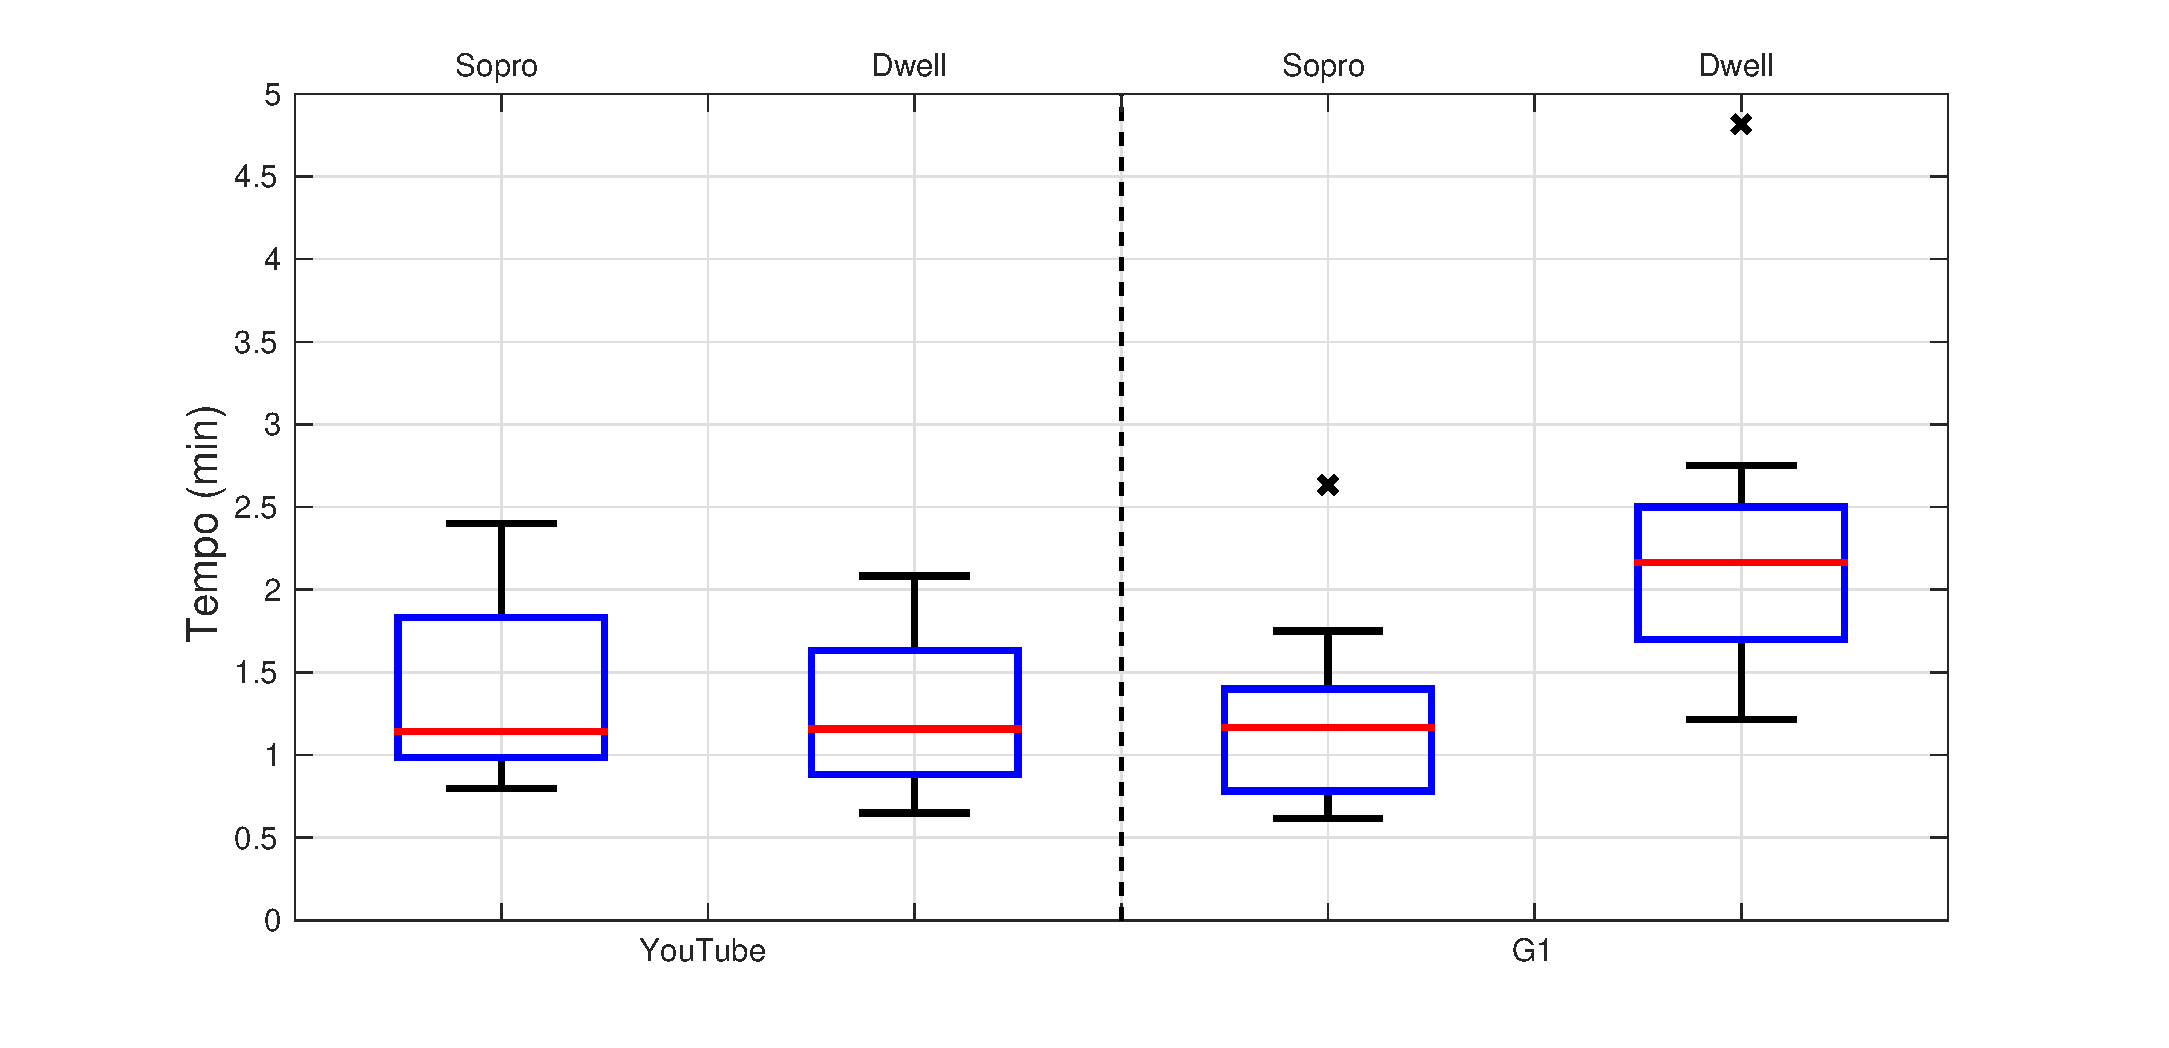
\includegraphics[width=1.0\linewidth]{fig/time}
	\caption{Distribuição do tempo de conclusão das tarefas.}
	\label{fig:tempo}
\end{figure}

Analisando a Figura~\ref{fig:tempo}, é possível perceber que, para o YouTube, o
\textit{dwell time} foi o método que a maioria das pessoas levou menos tempo
para completar a tarefa. Isso pode ser percebido pela amplitude das ``caixas''.
A maioria das pessoas precisou de 50 segundos (50s) a 1 minuto e 40 segundos
(1m40s) para terminar a tarefa do YouTube. Contudo, com o dispositivo baseado em
sopro, a maioria das pessoas levou de 1min a 1min50s para concluir a tarefa.

Por outro lado, para o \textit{website} G1, os participantes levaram mais tempo
para finalizar a tarefa utilizando o dispositivo de sopro. A maioria precisou de
45s a 1min30s para terminar a tarefa do G1. Apenas uma pessoa levou quase 3
minutos para concluir as tarefas do G1, o que explica o valor de
\textit{outlier} exibido como um ``x'' acima da respectiva ``caixa'' do G1. Com
o \textit{dwell time}, na tarefa do G1, também houve um caso \textit{outlier}
onde um voluntário completou a tarefa em quase 5 minutos (representado por um
segundo marcador em ``x''), no entanto, a maioria dos participantes finalizou a

Como o primeiro método de interação não convencional para o clique esquerdo do
\textit{mouse} foi o dispositivo de sopro, os participantes estavam mais
familiarizados quando as tarefas foram executados pela segunda vez (utilizando o
\textit{dwell time}). Isso pode ser observado no tempo em que os usuários
gastaram para executar a tarefa do YouTube onde o \textit{dwell time} foi o
método alternativo de clique em que  os participantes levaram menos tempo para
concluir a tarefa. No entanto, para o G1, mesmo os participantes já sabendo
exatamente todos os passos do tarefa, visto que eles já a tinham executado
anteriormente com o dispositivo de sopro, o tempo for muito maior com o
\textit{dwell time}. Isso aconteceu porque o G1, assim como diversos outros, não
é adaptado para tecnologias alternativas que usam o \textit{dwell time} como
método de clique dificulta demais a seleção correta dos itens desejados nesse
\textit{website}, especialmente devido a proximidade entre os itens, que são
expandido apenas passando o ponteiro do mouse sobre eles.
\end{subsection}

\begin{subsection}{Quantidade de Cliques}

A Figura~\ref{fig:cliques} mostra a quantidade de erros de clique (cliques
involuntários ou sem sucesso), feitos pelos usuários em cada tarefa. Alguns
participantes realizaram a tarefa do YouTube usuando o \textit{dwell time} sem
erros de cliques, representado pela caixa em azul a partir do zero, fato que não
aconteceu com a ferramenta baseada em sopro. No entanto, na tarefa do G1,o
número de erros aumentou consideravelmente no \textit{dwell time}, onde a
maioria dos voluntários errou entre 4 a 12 vezes.

\begin{figure}[!h]
	\centering
	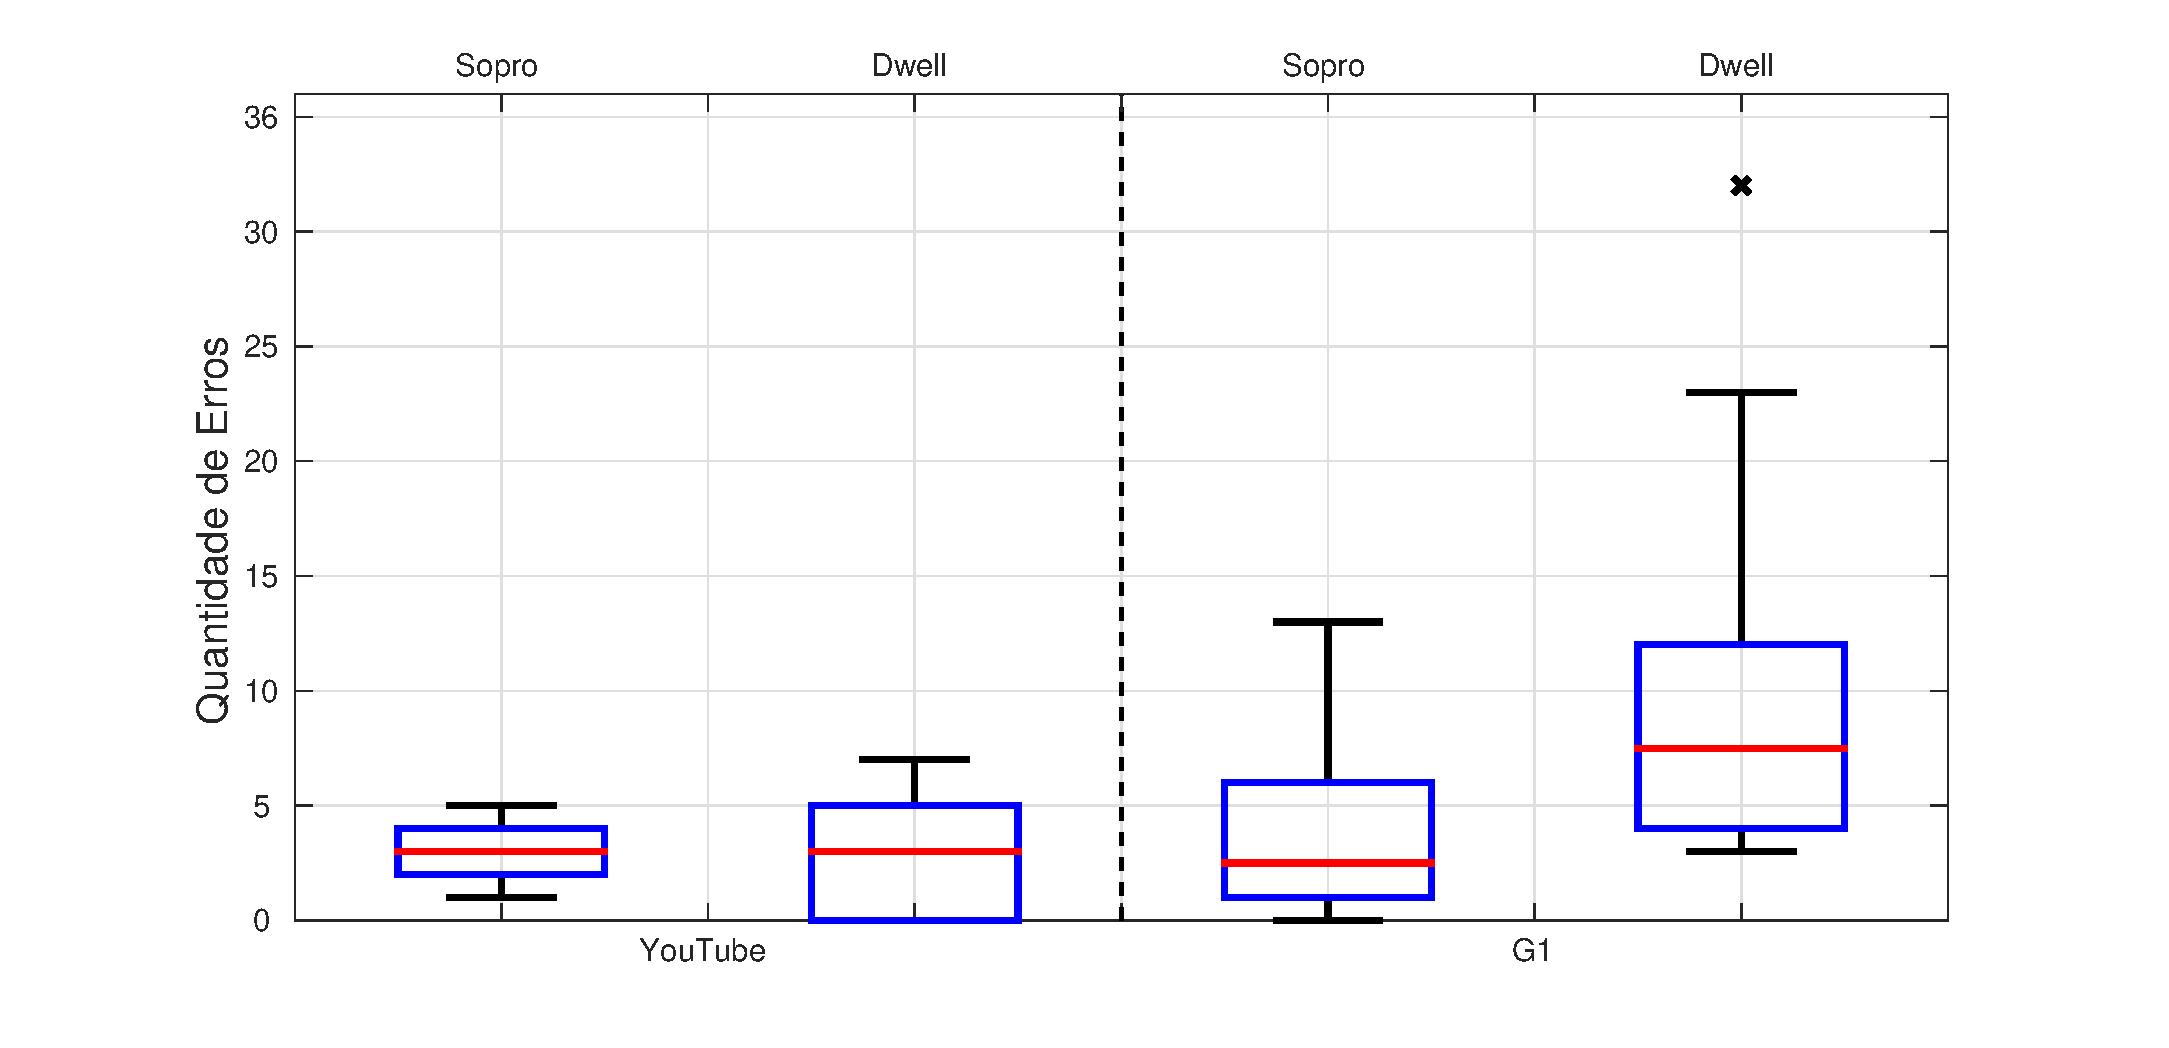
\includegraphics[width=1.00\linewidth]{fig/erros}
	\caption{Distribuição da quantidade de erros cometidos em cada tarefa.}
	\label{fig:cliques}
\end{figure}

A maioria dos dos erros de cliques cometidos pelos participantes com o
dispositivo baseado em sopro foi causado por cliques sem sucesso, onde a pessoa
soprava diretamente no transdutor piezoelétrico e o clique não ocorria. Isso
aconteceu principalmente no YouTube, visto que essa tarefa foi a primeira a ser
realizada pelos participantes e eles não sabiam ainda exatamente a intensidade
correta de sopro para que o clique ocorresse. Isso não aconteceu com o
\textit{dwell time}, visto que a função de clique é ativada depois de um certo
tempo em que o cursor do \textit{mouse} fica sobre uma mesma área. Portanto todo 
os erros cometidos pelos participantes utilizando o \textit{dwell time} foram
devidos a cliques involuntários.

As Figuras~\ref{fig:dwellclicks} e~\ref{fig:puffclicks} mostram a quantidade
total de cliques executados pelos usuários utilizando o \textit{dwell time} e o
dispositivo baseado em sopro, respectivamente. A quantidade mínima necessária
para a conclusão das duas tarefas era de seis cliques para a tarefa do YouTube e
quatro cliques para a tarefa do G1. Foram considerados apenas os cliques
realizados corretamente, assim como a quantidade de cliques involuntários e
cliques errados (quando o usuário clicava em itens que não estavam previstos nas
tarefas).


É importante notar que eViacam apresentou alguns problemas de detecção do rosto
do participantes, que afetaram diretamente na quantidade de cliques realizados.
A detecção de face falhou em quase diversos casos onde o participante tentou
posicionar o ponteiro do mouse nos cantos da tela. À medida que o cursor se
aproximava dos cantos, a velocidade no movimento do cursor (controlada pelo
rastreador de face do eViacam) diminuía, o que causou muitos cliques
involuntários quando os usuários estavam realizando as tarefas com o
\textit{dwell time}, visto que o cursor ficava sobre uma determinada área em
tempo suficiente para que a ação de clique fosse executada.

\begin{figure}[!h]
	\centering
	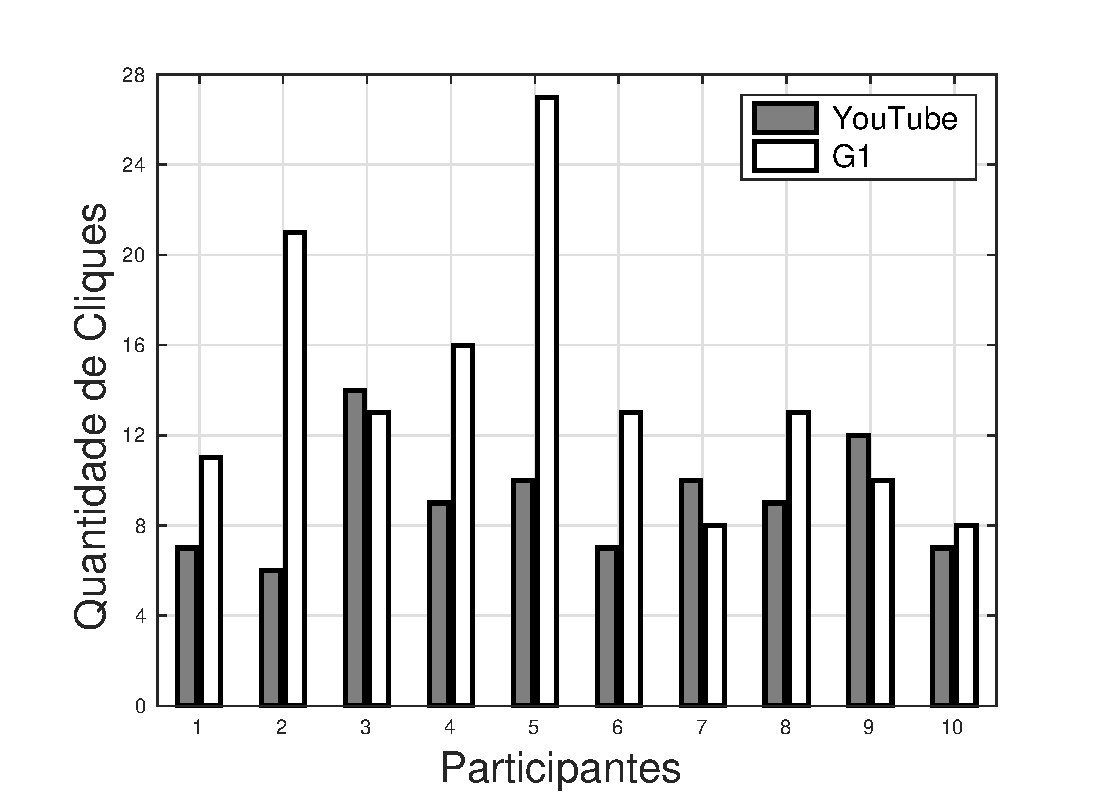
\includegraphics[width=1.00\linewidth]{fig/DwellClicks}
	\caption{Distribuição da quantidade de erros cometidos em cada tarefa.}
	\label{fig:dwellclicks}
\end{figure}

A quantidade de cliques quando os usuários utilizaram o \textit{dwell
time}~\ref{fig:dwellclicks} foi bastante alta. No total, 90\% dos participantes
não conseguiram concluir a tarefa do YouTube com o valor mínimo de cliques
estipulados (seis cliques). A situação piorou na tarefa o G1, uma vez que nenhum
participante conseguiu terminar a tarefa realizando apenas a quantidade mínima
de cliques e a média de cliques foi bem alta: 14 cliques para uma tarefa que
exigia apenas quatro.

A quantidade de cliques foi maior na tarefa do G1 devido a precisão,
relativamente alta, necessária para selecionar os pontos desejados. O voluntário
tentava clicar em ``economia'', mas acabava clicando no item ``educação'' devido
a grande proximidade desses itens localizados no menu do \textit{website}
(veja a Figura~\ref{fig:g1}). Isso ocorreu com diversos participantes que muitas
vezes ficaram frustrados por não conseguir clicar no item desejado.

\begin{figure}[!h]
	\centering
	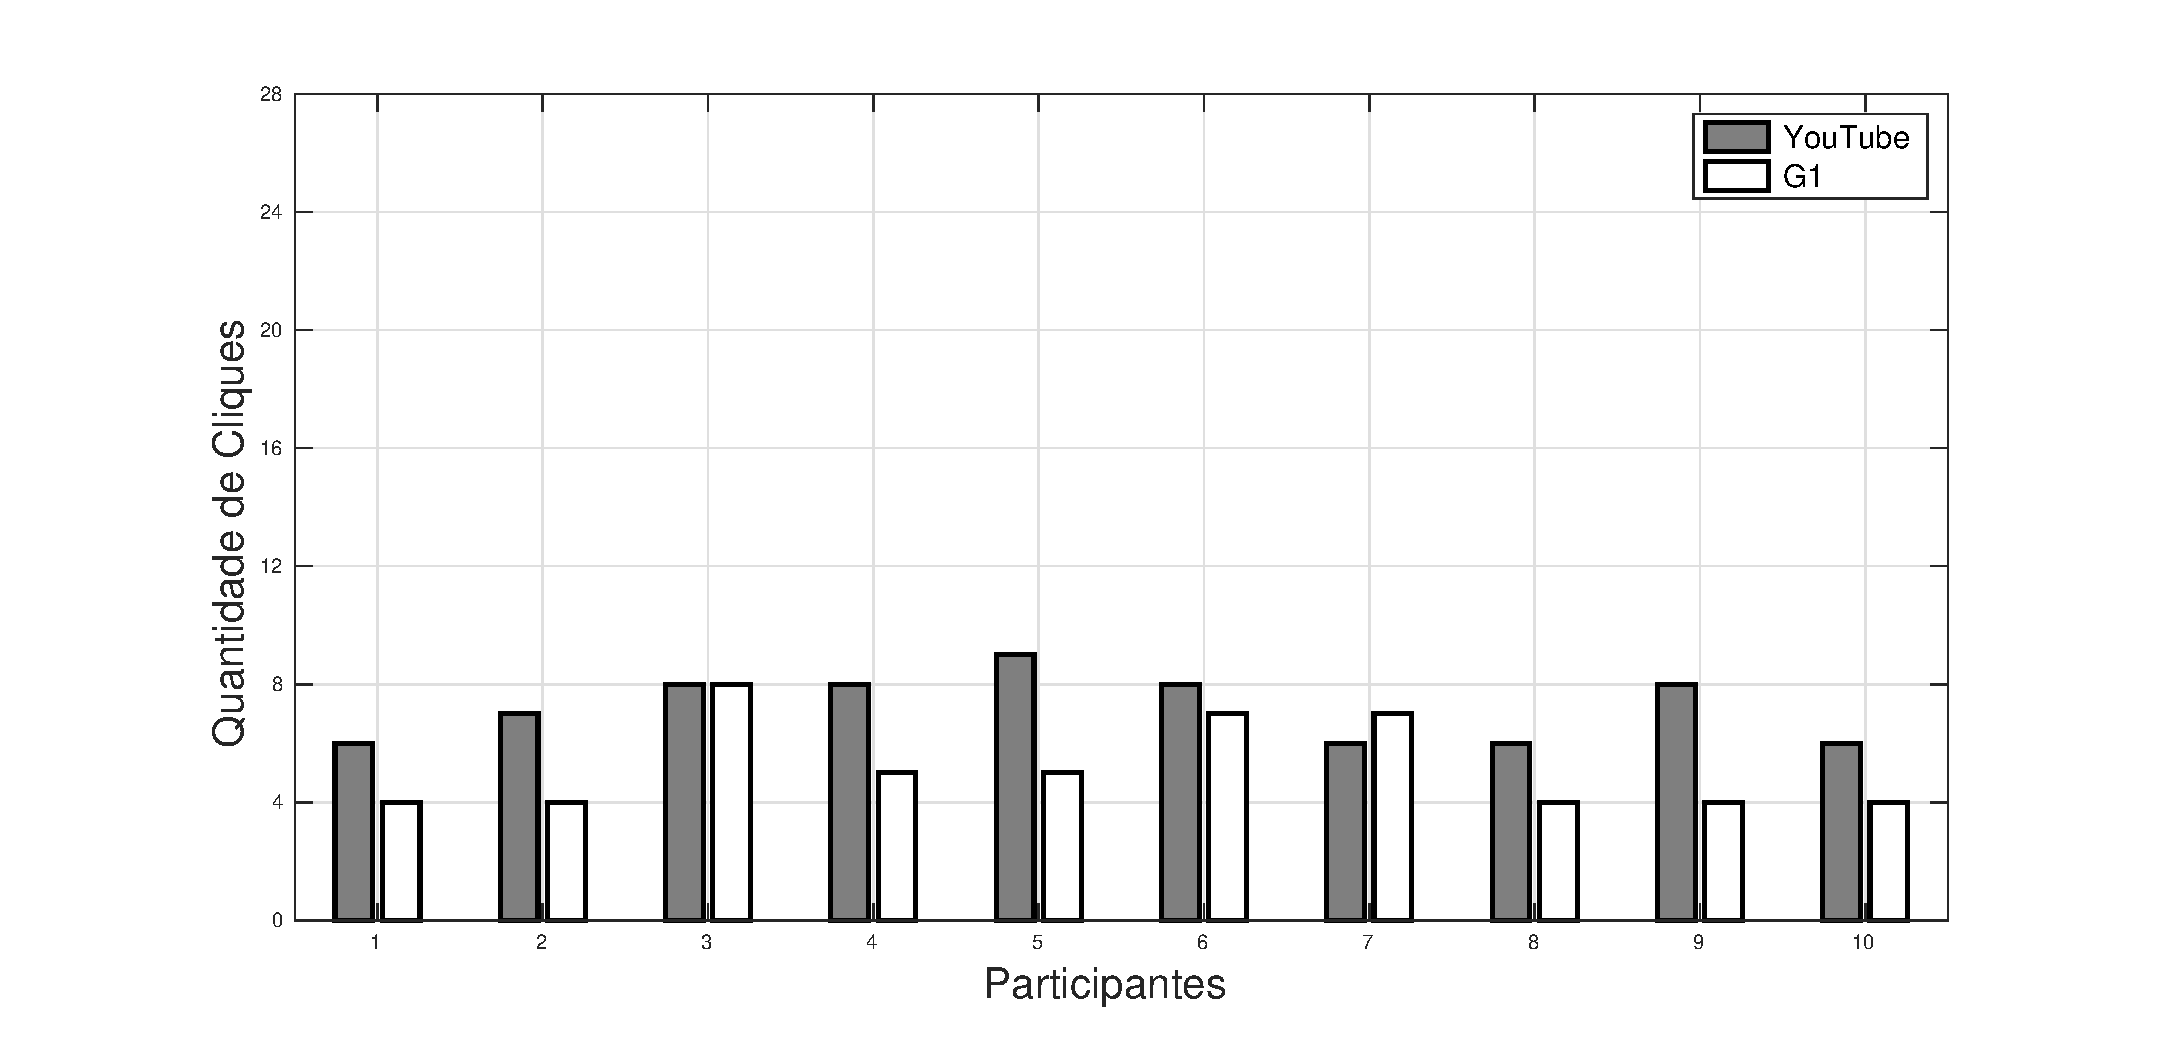
\includegraphics[width=1.00\linewidth]{fig/PuffClicks}
	\caption{Distribuição da quantidade de erros cometidos em cada tarefa.}
	\label{fig:puffclicks}
\end{figure}

No entanto, com o dispositivo baseado em sopro, os participantes realizaram
menos cliques do que com o \textit{dwell time}, como pode ser visto na
Figura~\ref{fig:puffclicks}. Na tarefa do YouTube, por exemplo, quatro pessoas
conseguiram concluir a tarefa utilizando somente seis cliques. No G1, 50\% das
pessoas completaram a tarefa utilizadno o número mínimo de cliques necessários,
enquanto que os demais precisaram de oito clique no máximo.

À primeira vista, o maior número de cliques ocorreu na tarefa do YouTube quando
os participantes utilizaram o protótipo baseado em sopro. Isso de fato
aconteceu, mas na verdade devido ao eViacam, que muitas vezes falhava em
detectar o rosto do participante durante a tentativa de posicionar o cursor nos
cantos inferiores do monitor, como relatado anteriormente.

Na tarefa do G1, por outro lado, a dificuldade foi novamente devido as áreas
clicáveis no menu desse \textit{website} estarem muito próximas umas das
outras. No entanto, notou-se que algumas pessoas moviam levemente a cabeça
enquanto sopravam, principalmente devido à força aplicada no peito durante a
expiração do ar. Consequentemente, o cursor do \textit{mouse} também se movia e
esse movimento era suficiente para que o ponteiro se movimentasse para outra
região, fazendo com que o usuário clicar em um alvo indesejado.
\end{subsection}

\begin{subsection}{Questões de Múltipla Escolha}
A seguir será mostrado os resultados das seis questões de múltipla escolha 
respondidas pelos voluntários. Essas questões pode ser vizualizada na
Tabela~\ref{tab:quest}.

\begin{table}[!h]
\centering
\small
\def\arraystretch{1.0}
\begin{tabular}{c|ll}
	\hline
	\hline
	 \textbf{Question} &\multicolumn{2}{c}{\textbf{Answer}} \\
	\hline
	 Como foi sua experiência usando esse método alternativo de clique? & 1 -- insuficiente        & 5 -- excelente   \\
	 O que você achou do tempo para realizar a tarefa?                  & 1 -- lento               & 5 -- rápido      \\
	 Como foi a precisão para realizar a tarefa?                        & 1 -- insuficiente        & 5 -- excelente   \\
	 Como foi o esforço cognitivo para realizar a tarefa?               & 1 -- alto                & 5 -- baixo       \\
	 Como foi o esforço físico para realizar a tarefa?                  & 1 -- alto                & 5 -- baixo       \\
	 Você se concentrou mais na tarefa ou no método de clique?          & 1 -- no método           & 5 -- na tarefa   \\
	%\hline
	%\textbf{\#}& \multicolumn{3}{c}{Based on your experience, what suggestions
	%would you give about the puff-based device?} \\
	\hline
	\hline
\end{tabular}
\caption{Perguntas utilizadas no questionário objetivo.}
\label{tab:quest}
\end{table}

As Figuras~\ref{fig:DwellQuestions} e~\ref{fig:PuffQuestions} mostram uma visão
geral de todas as respostas do questionário de múltipla escolha dadas pelos
participantes. Foi utilizado a escala Likert para representar as respostas, que
variam de 1 a 5, tanto para o \textit{dwell time} quanto para o dispositivo
baseado em sopro.  A resposta 1, colorida em vermelho, significa muito ruim,
enquanto que a resposta 5, colorida em verde escuro, significa muito bom. Ao
realizar um rápida comparação entre as respostas é possível afirmar que os
participantes se sentiram mais satisteitos com o desempenho geral do dispositivo
de sopro do que com o \textit{dwell time}, uma vez que a maioria das respostas
para o método de clique baseado em sopro em ambas as tarefas realizadas foram 4
ou 5, como mostrado na Figura~\ref{fig:PuffQuestions}, enquanto que as respostas
para o \textit{dwell time} variaram de 3 a 5, como mostrado na
Figura~\ref{fig:DwellQuestions}.  

\begin{figure}[!h]
	\centering
	\begin{minipage}[c]{\textwidth}
	\centering
	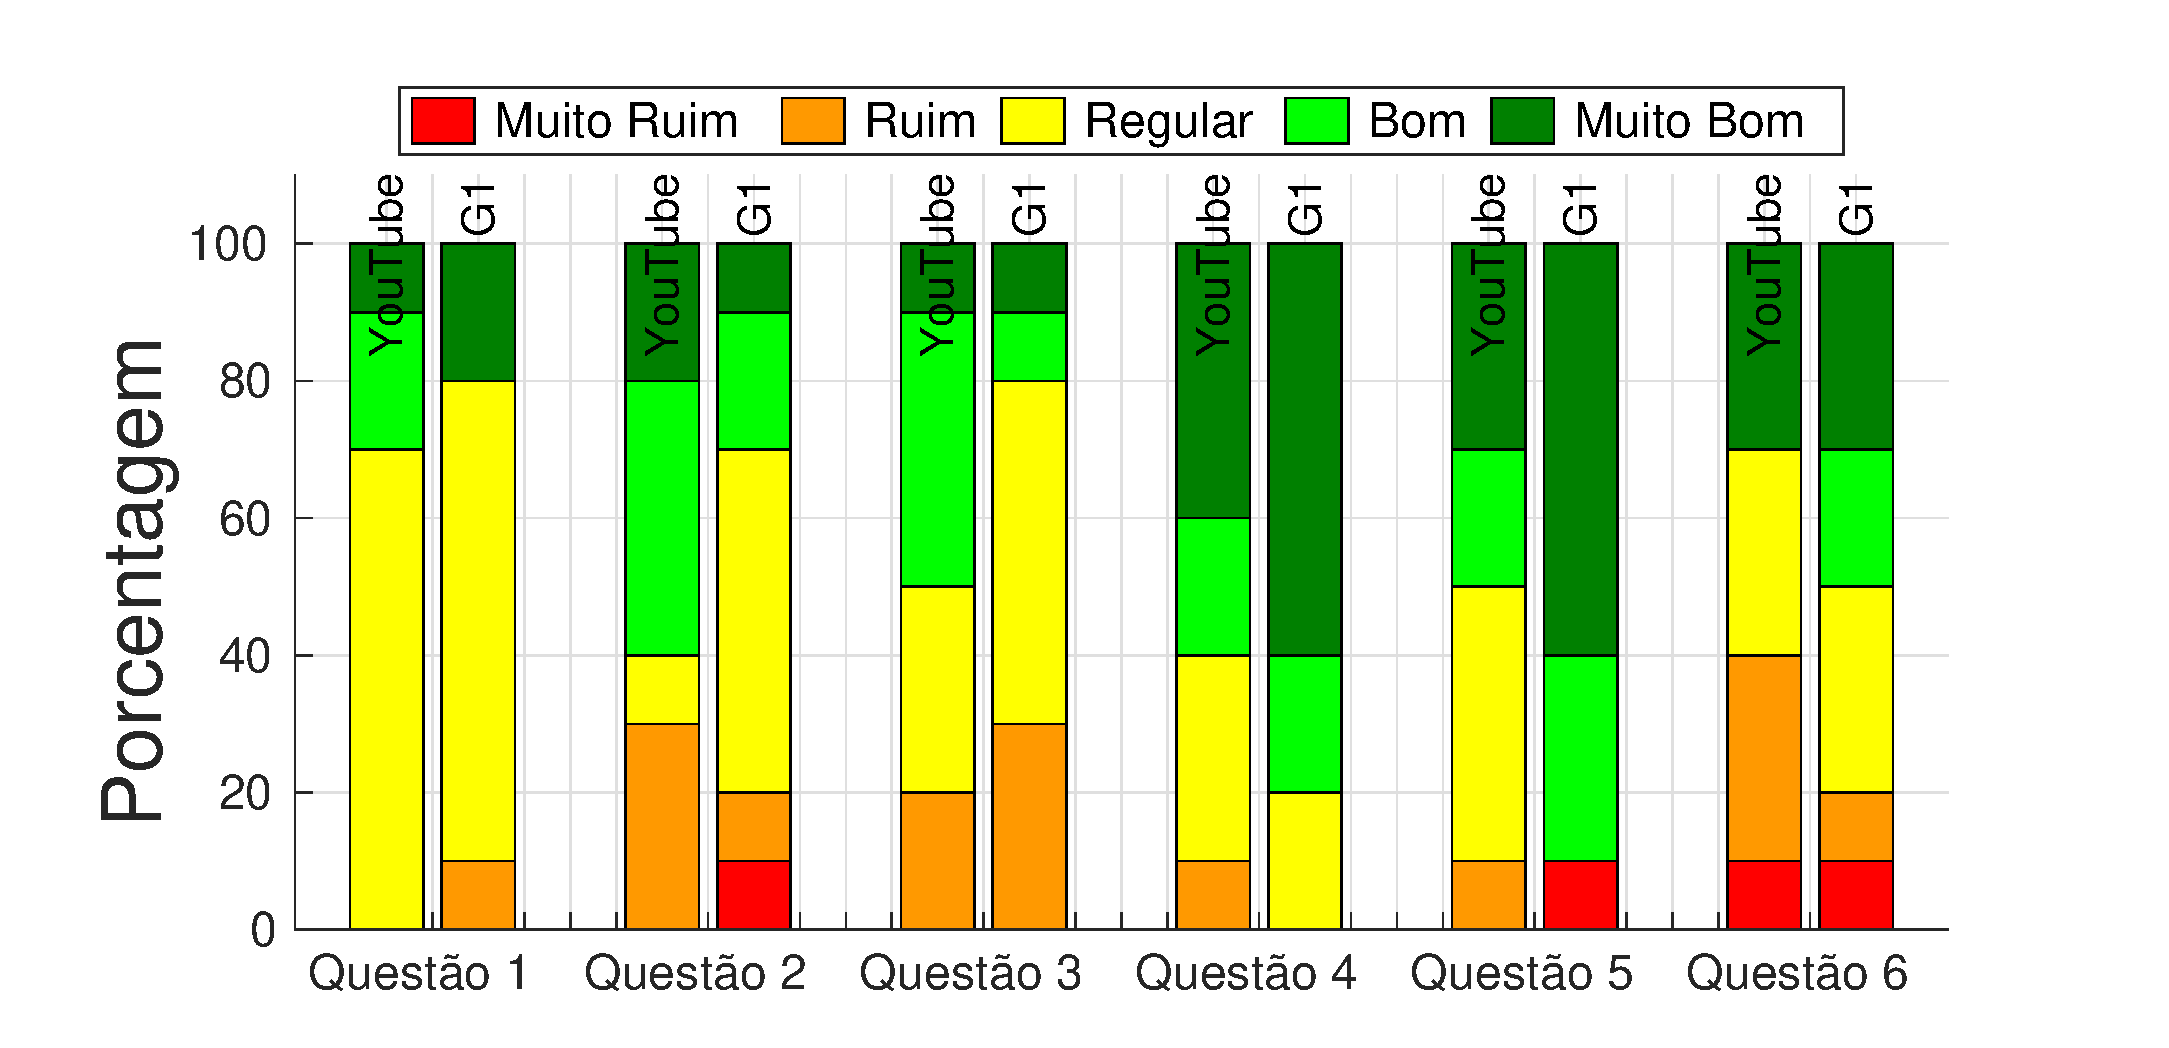
\includegraphics[width=0.9\linewidth]{fig/DwellQuestions}
	\caption{Likert scale of the dwell time questions.} 
	\label{fig:DwellQuestions}
	\end{minipage}
\end{figure}

\begin{figure}[!h]
	\centering
	\begin{minipage}[c]{\textwidth}
	\centering
	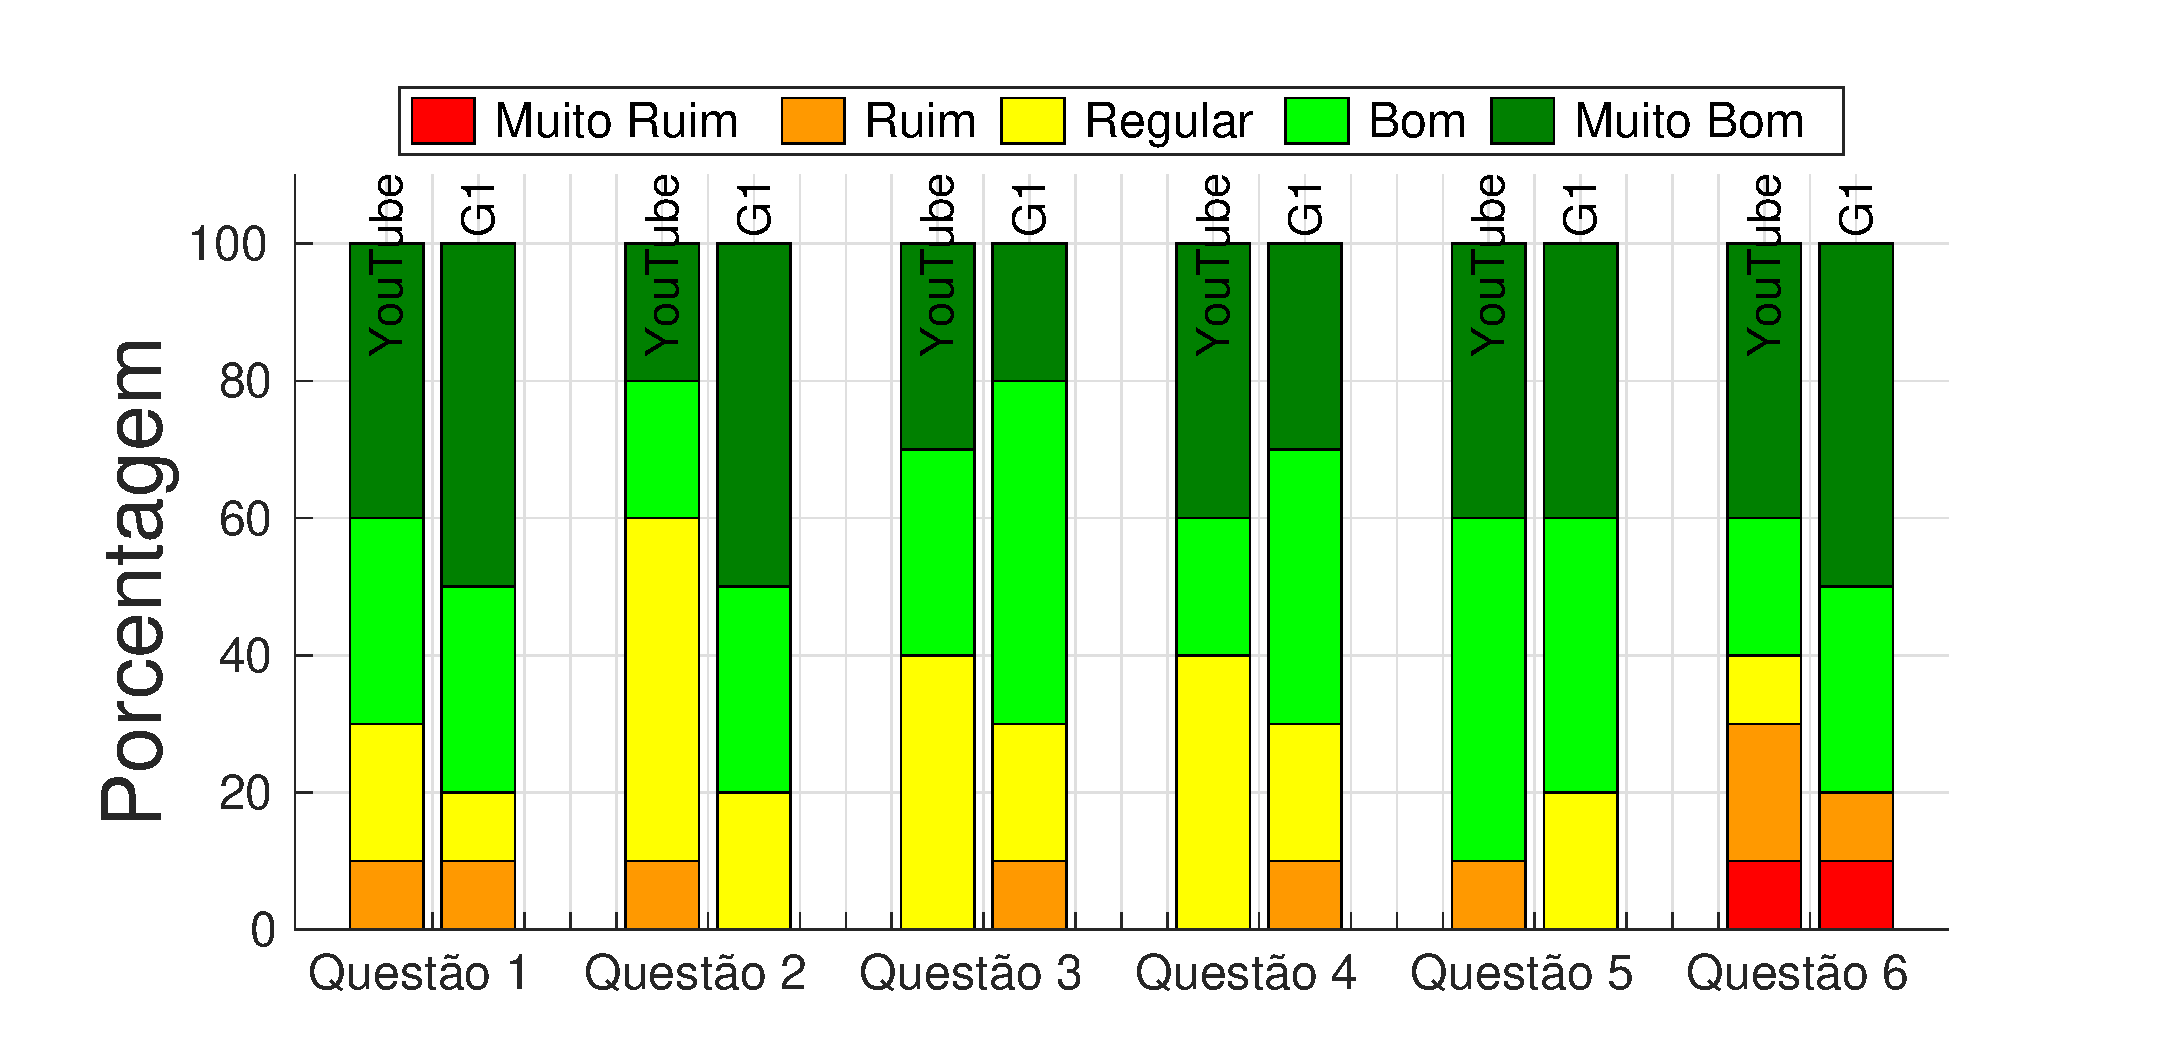
\includegraphics[width=0.9\linewidth]{fig/PuffQuestions}
	\caption{Likert scale of the puff questions.}
	\label{fig:PuffQuestions}
	\end{minipage}
\end{figure}



É notório a quantidade superior de respostas que variaram de 1 a 3 para o
\textit{dwell time} em comparação com o clique baseado em sopro, o  que
significa a maioria das pessoas não ficara, tão satisfeitas com o desempenho do
\textit{dwell time}. De acordo com os participantes, essa insatisfação ocorreu
principalmente devido a tarefa do G1 ser considerada mais problemática de ser
realizada utilizando o \textit{dwell time}, visto que eles precisaram mover o
cursor do \textit{mouse} mais lento que o normal devido a proximidade dos itens
clicáveis localizados no menu do \textit{website}. Diversas vezes a lentidão do
ponteiro do \textit{mouse} provocou clique involuntários devido o cursor estar
sobre uma determinada área por tempo suficiente para a ocorrer a ativação do 
clique.

Na questão 1, os usuários relataram que a exeperiência de uso, com o
\textit{dwell time}, foi regular, como pode ser percebido pela maior
concentração de retângulos em amarelo para ambas as tarefas realizadas. Com o
dispositivo baseado em sopro, por utro lado, a experiência de uso foi
considerada boa, visto que mais de 60~\% dos participantes responderam 4 ou 5.
Quanto ao tempo gasto para realizar uma tarefa, perguntado na questão 2,
anlizando apenas a tarefa do G1, novamente os usuários apontaram que o clique
realizado com o dispositivo baseado em sopro foi melhor, uma vez que apenas
30~\% dos participantes deu uma resposta abaixo de 3, um fato que não ocorreu
para o clique realizado com o \textit{dwell time}.

Os participantes também não ficaram satisfeitos com a precisão do \textit{dwell
time}, já quqe apenas 20~\% dos voluntários deu nota 4 ou 5 para a pergunta 3 na
tarefa do G1. No YouTube, os participantes não tiveram dificuldade em realizar a
tarefa, visto que não era necessário uma grande precisão para executá-la. 

O esforço cognitivo, perguntado na questão 3, foi muito similar para ambos os
métodos de clique. Contudo, analizando a questão 5, que perguntava sobre o
esforço físico para realizar as tarefas, é possível notar que na tarefa do
YouTube, o dipositivo baseado em sopro provocou menos esfoço físico nos
participantes, pois 90~\% das respostas foram 4 ou 5 enquanto que apenas 50~\%
das repostas foram 4 ou 5 para o \textit{dwell time}. Já na tarefa do G1
aconteceu o contrário: o \textit{dwell time} foi o método que necessitou de menos
esforço físico para realizar a tarefa, pois 60~\% das respostas foi 5 e outros
30~\% das respostas doi 4. Essa quantidade foi maior que as repostas para o
método de clique baseado em sopro, onde 40~\% dos usuários respondeu 5 e outros
40~\% respondeu 4.

A razão pela qual o método de clique baseado em sopro exigir mais esforço físico
para realizar a tarefa do G1 pode ser a dificuldade que os voluntários tiveram
em realizar a ação de sopro sem movimentar muito a cabeça. Como os itens do menu
do G1 são bastantes próximos uns dos outros, alguns movimentos (incluindo os
executados durante a inalação e exalação do ar ao executar a ação de sopro, 
que afeta praticamente todo o torso humano), deslocavam o ponteiro do alvo
desejado.

Por fim, é possível observar na última questão que os participantes se sentiram
mais à vontade ao utilizar o dispositivo baseado em sopro, pois a maioria
resposndeu 4 ou 5, o que significa que os vonluntários se concentraram mais na
realização da tarefa do no método de clique. Esse fato não se confirmou com o
\textit{dwell time}, pois a maioria das respostas variou de 1 a 3, ou seja, esse
método de clique interferiu na oncentração dos participnates na realuzação das
tarefas. 

\end{subsection}

\begin{subsection}{Discussão Sobre a Questão Subjetiva}

No final dos testes cada participnates foi convidado a responder em um
formulario virtual a seguinte pergunta: ``Com base na sua experiência de uso,
que sugestões você daria para melhoria do dispositivo baseado em sopro?''. Eles 
foram instruídos a se sentirem completamente livres para escrever críticas e 
apontar sugestões para a melhoria do dispositivo proposto. Todas as respostas
foram lidas e serão sintetizadas a seguir.

O maior problema identificado pela maioria dos participantes foi uso do
\textit{software} eViacam. A falha no rasteamento da face do usuário ao
posicionar o cursor do \textit{mouse} nos cantos da tela e em ícones pequenos
frustrou os participantes, que sugeriram a troca do \textit{software} de
controle do ponteiro do \textit{mouse}.

O dipositivo baseado em sopro proposto neste trabalho foi considerado uma boa
ferramenta para ser utilziada como um método alternativo de clique. Apesar do
bom desempenho do protótipo desenvolvido, houveram alguns problemas encontrados
pelos participantes, principalmente no que diz respeito a cliques involuntários.
Os voluntários sugeriram a substituição do \textit{headset} utilizado como
suporte para manter o protótipo desenvolvido próximo à boca do usuário, pois os
choques mecânicos causados pelo suporte utilizado geraram cliques involuntários.

Houveram também alguns casos onde o participante realizou a ação de sopro e o
clique não ocorreu. Isso ocorreu devido a intensidade do sopro não ser
suficiente para a ativação do clique. Para a maioria dos participantes a
sensibilidade do dispositivo baseado em sopro estava adequada, pois era
necessário um sopro relativamente fraco para a ativação do clique. No entanto,
alguns voluntários relataram que eles se sentiriam mais confortáveis se a
sensibilidade fosse aumentada. Há um potenciômetro acoplado no dispositivo
proposto que permite o ajuste da sensibilidade, porém apesar de estar ajustado
em um valor que não necessitava um sopro muito forte nem muito fraco, essa
sensibilidade gerou desconforto entre alguns usuários. A sugestão dada pelos
participantes foi a disponibilidade de três níveis de ajuste da sensibilidade
para que cada usuário possa escolher a intensidade de sopro ideal. Eles também
enfatizaram que o  dispositivo poderiam ter um \textit{feedback} visual afim de
mostrar para o usuário qual o nível de sensibilidade está definido no momento.


\end{subsection}

\end{section}

\end{chapter}
